%-----------------------------------------------------------------------------------
%	PACKAGES AND OTHER DOCUMENT CONFIGURATIONS
%----------------------------------------------------------------------------------

\documentclass[11pt]{article}

\usepackage[top=2cm, bottom=3cm, left=2cm, right=2cm]{geometry}
\setlength{\parskip}{1em}
\setlength{\parindent}{4em}
\linespread{1.25}

\newcommand{\Var}{\mathrm{Var}}

\newcommand{\Cov}{\mathrm{Cov}}

\newcommand{\plim}{\rightarrow_{p}}

\usepackage{apacite}

\usepackage{amsmath, amsfonts}
\usepackage{graphicx}
\usepackage{pdfpages}
\usepackage{bm}
\usepackage{listings}
\usepackage{multirow,array}
\usepackage{enumerate}
\usepackage{bbm}
\usepackage{subfig}
\usepackage{bbm}

\usepackage[latin1]{inputenc}

\usepackage{amssymb}

\usepackage{mathrsfs}
\usepackage{float}
\usepackage{booktabs}
\usepackage{color}
\usepackage{rotating}
\usepackage{amsthm}
\usepackage{multirow,array}
\usepackage{caption}
\usepackage{url}



\DeclareMathOperator*{\argmax}{arg\,max}
\DeclareMathOperator*{\argmin}{arg\,min}



% Expectation symbol
\newcommand{\E}{\mathrm{E}}
\newcommand{\V}{\mathrm{V}}
\newcommand{\N}{\mathcal{N}}
\newcommand{\R}{\mathbb{R}} 

%----------------------------------------------------------------------------------
%	TITLE AND AUTHOR(S)
%----------------------------------------------------------------------------------

\title{Marijuana Access and Alcohol Use } % The article title

\author{Nathan Mather} % The article author(s) 

\date{\today} % An optional date to appear under the author(s)

\renewcommand{\contentsname}{Table of Contents}
%----------------------------------------------------------------------------------
\begin{document}
	
	
%------------------------------------------------------------------------------
%	TABLE OF CONTENTS
%------------------------------------------------------------------------------
\maketitle % Print the title/author/date block

\setcounter{tocdepth}{3} % Set the depth of the table of contents to show sections and subsections only

\tableofcontents % Print the table of contents

%------------------------------------------------------------------------------
% Introduction 
%------------------------------------------------------------------------------
\section{Introduction}
\subsection{Motivation}

In 2012 Colorado and Washington voted to legalize recreational marijuana in a bold move that defied federal laws.  While there was some uncertainty around how the federal government would react and if recreational dispensaries would be allowed to operate, in terms of bucking federal law, offering legal recreational marijuana, and collected tax revenue, this experiment proved to be a success. In 2014, the first year recreation dispensaries opened, Colorado had \$683,523,739 in sales and \$67,594,323 collected in taxes \cite{Colorado_marijuana_sales}. California , D.C., Maine, Massachusetts, Nevada, Oregon, Vermont, Washington, and Michigan have all followed suit since and enacted some form of legal recreational marijuana. These policies have been a success in terms of implementing their stated goals, but what has the impact of readily accessible marijuana been on public health? \par

There are a variety of factors that influence this question, but one key component is how easier access to marijuana will affect the consumption of alcohol. While there is much debate about the extent to which marijuana causes public harm, there is little doubt that increased consumption, all else equal, will come with some costs. While the impact of marijuana on individual health is still in need of additional research, marijuana can impair motor skills and can lead to traffic fatalities \cite{webmd_mj}. Of course, all else is not equal.  Despite potential harmful effects, if marijuana acts as a substitute for alcohol, which may have more serious negative public health impacts, the general equilibrium effect may be a public health win. If Marijuana is a compliment to alcohol, however, then legalization of marijuana may increase the negative impacts of alcohol. \par


There are many concerns unrelated to public health that come into play in the normative discussion around marijuana legalization. I do not think that knowing the relationship between alcohol and marijuana will end this discussion; however, increasing our understanding of the implications of legalization will give policy makers a clearer picture of the costs and benefits involved and may help guide specific policy to ensure a smooth rollout of marijuana legalization policies.




\subsection{Existing Literature}

The existing literature on the relationship between recreational marijuana legalization and alcohol consumption is fairly limited. Most of the published work either considers the relationship between marijuana and alcohol through the lens of medical marijuana or does not focus on the impact recreational marijuana has specifically on alcohol.\par 


A paper by Baggio, Chong, and Kwon addresses the substitutability of marijuana and alcohol by using retail scanner data and variation in medical marijuana laws. They use a fixed effects model of counties across the United States over time. Their variable of interest is if the county has medical marijuana or not. They find that counties located in states that allow medical marijuana reduced monthly alcohol sales by 15 percent" \cite{baggio_chong_kwon_2018}. I use a similar approach to examine the impact of recreational marijuana. I also use the retail scanner data, but in addition to marijuana laws I consider the geographic distribution of marijuana retailers within a state over time. While legalization increases access, it's effects are likely different if a retail location is readily available. \par


The above paper and the approach I take below are light on theory. However, a paper by Miller and Seo, which analyzes the complementarity of marijuana and alcohol in the context of tax revenues, uses a more structural theory driven approach. To set up this problem they use a multistage budgeting approach. The top stage is substances. The second stage is Marijuana, alcohol, or tobacco. Finally, the third stage is which types of each product to consume, beer or wine for example. They estimate their model using the Nielson Scanner data and data on sales and prices of marijuana directly from the state of Washington. To account for endogeneity of prices when estimating demand, they use wages and county and time fixed effects as an instrument for prices as well as wholesale prices and taxes.  They cast doubt on the validity of using surrounding states as a control since Oregon saw significant alcohol price changes around the time of marijuana legalization. They instead use price changes within Oregon after legalization along with this model to tease out this relationship \cite{miller_seo_2018}. \par


While their approach incorporates prices and does not rely on comparing states that differ in potentially unaccounted for ways, there are other issues with their specification. Most importantly their estimation strategy requires estimating the actual quantity of marijuana consumed. They point out themselves that prior to legalization an estimated 85 to 225 metric tons of marijuana were sold in Washington while only 29 metric tons were sold after legalization \cite[p.~13]{ miller_seo_2018}.  While they try to explain away the difference with varying THC concentrations, it is not a convincing argument for this dramatic of a difference. Additionally, we would actually expect new customers from out of state coming into Washington and inflating sales. Making the 29 ton number seem especially small. \par


Miller and Seo also run into problems because they need prices for their equations, but prices are endogenous to the demand for products. They attempt to solve this problem by instrumenting for prices. By using the shock of legalization and subsequent opening of retail locations I avoid this problem. While states that legalize marijuana likely have more demand for drugs in general, including alcohol, I do not expect it was a sudden shock to demand for alcohol or marijuana right before legalization that led to marijuana legalization. Rather, it was pressure over time from existing support in the state. These long-term differences can be captured with fixed effect and should not bias direct estimates of the impact of legalization. By considering a policy specific shock, however, I lose the level of precision that allows Miller and Seo to estimate an actual cross price elasticity. Instead, I get a coefficient based on a policy specific parameter like legalization. The direction, however, should not change. 





\subsection{Outline}



I have considered multiple analytical approaches and data sources to address the impact of legalization and readily accessible marijuana on alcohol consumption. the remainder of this paper proceeds as follows. First, I discuss the theoretical approach I am using to answer this question. Specifically, I explain why The event of legalization and opening of dispensaries has sound theoretical footing to address this question. Next, I discuss the data sources I use. These include the CDC's Behavioral Risk Factor Surveillance System survey, the Nielson Scanner data, and geographic data on dispensary locations. After reviewing the data, I  walk through the analytical methods I employ and discuss the results. Finally, I discuss the shortcomings and areas of improvement for my paper and how I hope to address these in the future. 

%------------------------------------------------------------------------------
% Theoretical Approach
%------------------------------------------------------------------------------

\section{Theoretical Approach}

I aim to determine the effect of marijuana legalization and readily accessible recreational marijuana on alcohol consumption. This policy specific question can also be stated using the basic theory of compliments and substitutes. That is, are marijuana and alcohol compliments or substitutes? \par


To answer this question  I rely on the assumption that legalization and recreational dispensaries lower the cost of consuming marijuana. This assumption comes from two aspects of recreational marijuana legalization and basic theory. The first is that legalization directly lowers the cost of consuming marijuana by eliminating the risk of legal repercussions. The second is that providing legal marijuana retailers lowers the inconveniences of purchasing marijuana from an individual rather than a retail location. \par

 Let the expected cost of purchasing and consuming illicit marijuana be C. If we are considering legalization alone then C is simply the costs or expected legal risks associated with purchasing an illegal substance. If we are considering legalization along with readily accessible retail marijuana dispensaries than C could also include the inconveniences of purchasing marijuana from an individual rather than a retail location with laws regulating trade. With this in mind, prior to legalization, consumers are effectively paying $P_B + C$, the black-market price plus the cost of illegal activity. Legalization will increase the marginal benefit of marijuana consumption by C. On its own, this would actually lead to an increase in the demand for marijuana and thus an increase in the market price and quantity; however, as figure 1 shows, the old effective price $ P_B + C$ is still greater than the new market price $P_E$ (which is also the effective price in the absence of legal repercussions). This leads to a reduction in the real price for consumers from $ P_B + C$ to $P_E$. If marijuana and alcohol are substitutes, this should decrease demand for alcohol even though the list price of marijuana is increasing.\par
\begin{center}
	\centering
	
	\textbf{Figure 1}\par\medskip
	
	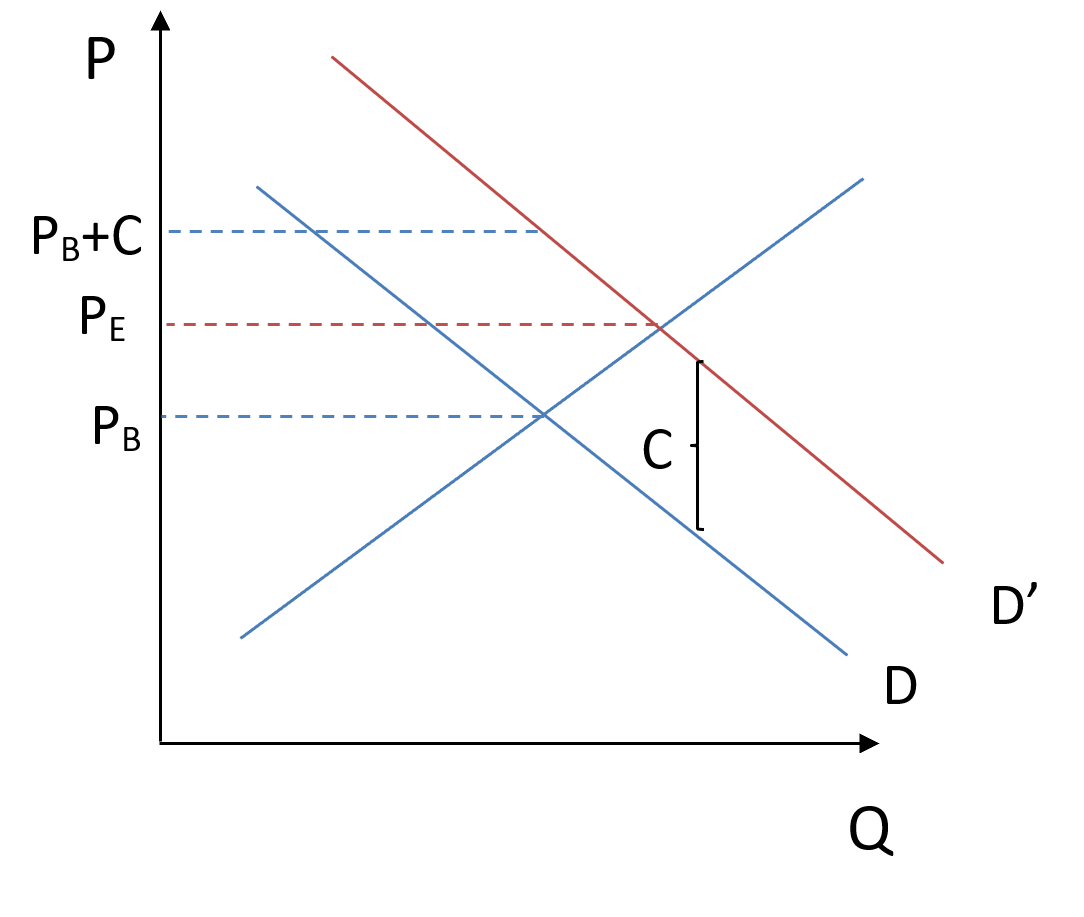
\includegraphics[width=.5\linewidth]{legal_dside.png}
	
\end{center}


In addition to the demand effect, legalization will also lower the marginal cost of production. Lower marginal costs for producers results in a basic shift to the right of the supply curve. As legal action against growers and suppliers is generally more harsh than for consuming small amounts, I suspect the magnitude of this shift will be large relative to the demand shift. Additionally, by allowing recreational dispensaries and formal businesses in marijuana production and distribution, economies of scale will further increase supply. This rightward shift in the supply curve also works to lower the price of marijuana to consumers. \par

Miller and Seo's approch ignores the cost $C$ and instead focuses on cross price elasticity for the price of marijuana in the legal market. This may be of interest after legalization has taken effect, but it is not helpful for determining the impact of legalization itself since it says nothing about the size of $C$ or the prcies of black market marijuana. \par


One objection that could be made to this claim is that price controls and burdensome regulation on the legalized production and sale may lead to a higher price for regulated marijuana than the prior price of black-market marijuana. It is important to remember, however, that the black market is still an option for producers and consumers. Taken to the extreme, regulation may be so burdensome that no dispensaries open and legalization does not shift supply to the right at all. In this case, however, the observed market price may be higher for consumers, but, as figure one shows, the effective price is still lower as the risk of legal repercussions has fallen. The exception to this would be if governments paired their legalization with a crackdown on black market trade, but we do not see this in practice. \par

Another potential objection is that these policy changes are not happening in isolation, and may in fact be correlated with increases in demand for either marijuana or alcohol from some other factor. I do not think this concern is warranted for the event of legalization. Take, for example, Colorado and Nebraska. Colorado likely has higher demand for marijuana and possibly alcohol too. However, I do not think that difference developed discreetly at the time of legalization. Rather, the higher demand and support for marijuana in Colorado over time led to legislative changes that occurred as a discrete event. When considering the availability of marijuana dispensaries, this objection is a bit more concerning, but I do not think it is of first order concern. In a typical market, demand shocks will lead to an increase in quantity supplied and, likely, an increase in in number of stores. In the market for marijuana immediately after legalization, however, I expect legal red tape, local zoning laws, funding, and uncertainty, are the primary forces impacting the accessibility of stores. And again, existing difference across areas can be remove with fixed effects. So, we need only consider changes to demand that correspond to the number of dispensaries, not differing overall levels of demand by region. \par


With the assumption that legalization of recreational marijuana will lower the effective price paid by consumers, I can appeal to the basic theory of compliments and substitutes. If marijuana and alcohol are compliments, we should see alcohol consumption rise as a result of the policy shocks. If they are substitutes, we should see alcohol consumption fall.\par




%------------------------------------------------------------------------------
% Data
%------------------------------------------------------------------------------

\section{Data}

In order to measure alcohol use I first turned to the state-based Behavioral Risk Factor Surveillance System (BRFSS) put out by the Centers for Disease Control and Prevention (CDC). it is "a cross-sectional telephone survey that state health departments conduct monthly over landline telephones and cellular telephones with a standardized questionnaire and technical and methodologic assistance from CDC" \cite{BRFSS_homepage}.The survey has a sample size of around 500,000 a year and covers the years 2011-2017. The survey includes two questions that together give average drinks per week. These include: how many days per week or per month did you have at least one drink of any alcoholic beverage such as beer, and how many drinks do you usually have when you drink. \par


I was initially very optimistic about this data. The BRFSS survey has the advantage covering all alcohol consumption for the individuals surveyed as well has having a large sample size. The survey also provides a rich set of covariates. In theory, this could offer a detailed look at alcohol use, but I have uncovered a number of issues. The biggest of which is measurement error. Alcohol consumption is a sensitive topic for many. Not only is there the possibility that some people intentionally misrepresent their consumption, but people may not even be able to honestly recount their use. While I expected people to constantly lie downwards and underreport their drinking habits, there are a number of extremely large outliers that must either be intentional misrepresentation or possibly entry errors. For example, there are entries of averaging over 70 drinks a day for 30 days out of the month. To deal with this I have truncated the data at the 99th percentile. This potentially biases the results, but it's also removing some clearly false data that would also bias the results; so, I think it is a reasonable strategy. Overall, if the measurement error is random it shouldn't systematically bias the results, since alcohol use is the dependent variable, but it may make it hard to detect a statistically significant result. \par

  The data also only includes respondents state of residence and is not a panel. This means I can only include state fixed effects and that the only variation in marijuana policies and access that occur is at the state level. The state level policy changes are summarized in the tables below. The medical Marijuana dates are a combination of the data from the cBaggio, Chong, and Kwon paper and news articles for later dates \cite{baggio_chong_kwon_2018}. The Recreational Marijuana dates are all obtained from various news articles.  \par

\begin{figure}[H]
	\centering
	\Large{\textbf{State Level Policy Changes}}\par\medskip
	\scalebox{.6}{
		% latex table generated in R 3.5.1 by xtable 1.8-3 package
% Mon Dec 17 06:05:16 2018
\begin{tabular}{lc}
  \hline
state & Date Recreational Marijuana Legalized \\ 
  \hline
alaska & 2015-02-24 \\ 
  california & 2016-11-09 \\ 
  colorado & 2012-12-10 \\ 
  district of columbia & 2015-02-26 \\ 
  maine & 2017-01-27 \\ 
  massachusetts & 2016-12-15 \\ 
  nevada & 2017-01-01 \\ 
  oregon & 2015-07-01 \\ 
  washington & 2012-12-06 \\ 
   \hline
\end{tabular}

	}
	\scalebox{.6}{
		% latex table generated in R 3.5.1 by xtable 1.8-3 package
% Mon Dec 17 06:05:16 2018
\begin{tabular}{lc}
  \hline
state & Date Medical Marijuana Legalized \\ 
  \hline
alaska & 1999-03-01 \\ 
  arizona & 2011-04-01 \\ 
  arkansas & 2016-11-01 \\ 
  california & 1996-11-01 \\ 
  colorado & 2001-06-01 \\ 
  connecticut & 2012-05-01 \\ 
  delaware & 2011-07-01 \\ 
  district of columbia & 2010-07-01 \\ 
  florida & 2017-01-01 \\ 
  hawaii & 2000-12-01 \\ 
  illinois & 2014-01-01 \\ 
  maine & 1999-12-01 \\ 
  maryland & 2014-06-01 \\ 
  massachusetts & 2013-01-01 \\ 
  michigan & 2008-12-01 \\ 
  minnesota & 2014-05-01 \\ 
  montana & 2004-11-01 \\ 
  nevada & 2001-10-01 \\ 
  new hampshire & 2013-07-01 \\ 
  new jersey & 2010-10-01 \\ 
  new mexico & 2007-07-01 \\ 
  new york & 2014-07-01 \\ 
  north dakota & 2016-12-01 \\ 
  oregon & 1998-12-01 \\ 
  ohio & 2016-08-01 \\ 
  pennsylvania & 2016-05-01 \\ 
  rhode island & 2006-01-01 \\ 
  vermont & 2004-07-01 \\ 
  washington & 1998-11-01 \\ 
  west virginia & 2017-07-05 \\ 
   \hline
\end{tabular}

	}
\end{figure}

While analyzing the BRFSS data is instructive, the issues uncovered warrant including an additional alcohol use measure and alternative analysis.  I also use Alcohol sales data from the Nielson Retail Scanner Data . Nielson collects alcohol sales directly from retailers on a weekly basis. Measuring alcohol use in this way does have some drawbacks compared to the BRFSS survey. Alcohol sales in bars and restaurants are completely left out of the sample. Additionally, we are limited to the retail chains that accept the survey. That being said, there is extensive coverage. The Figure in Appendix A shows the number of counties with sales data per month in an unbalanced panel going from 2011 to 2016. It is roughly 1900 counties per month. I drop any counties that are in less than ten months of data because I use county fixed effects in the model for this data \footnote{There are less that 100 counties that get dropped}. I only use data going back to 2011 even though the scanner data goes back to 2006 because recreational marijuana does not take place in any state until 2014. I wanted to limit the amount of pre-treatment data to a more reasonable level. This was done in an ad-hoc way because the fixed effect model should account for pre and post time trends, but I don't want to stretch the assumptions too far. The Data ends in August of 2016 because in September of 2016 the first recreational marijuana dispensaries opened in Oregon. I only have dispensary data for Washington and Colorado, so I cut the time series 3 month short of the full Nielson sample. July 2014 was missing from the Colorado dispensary geography data so I exclude that month as well. \par

The Geographic dispensary data comes from the Washington State Liquor \& Cannabis Board and the Colorado Department of Revenue Enforcement Division. The data sources give me a monthly snapshot of every licensed retailer and their address. Using the Texas A\&M Geocoding services I convert these address into latitude and longitude coordinates \cite{tamu}.To determine what county each dispensary is in as well as each dispensary's distance to each county I use the Cartographic County Shape files from the United States Census Bureau \cite{branch_2018}. Figures 2 and 3 show the evolution of marijuana dispensaries in Colorado and Washington over time. We can see that the number of dispensaries stabilized more quickly in Colorado while Washington has had a slower expansion. \par


\begin{figure}[H]
	\centering
		\LARGE{\textbf{Figure 2}}
	\subfloat{
		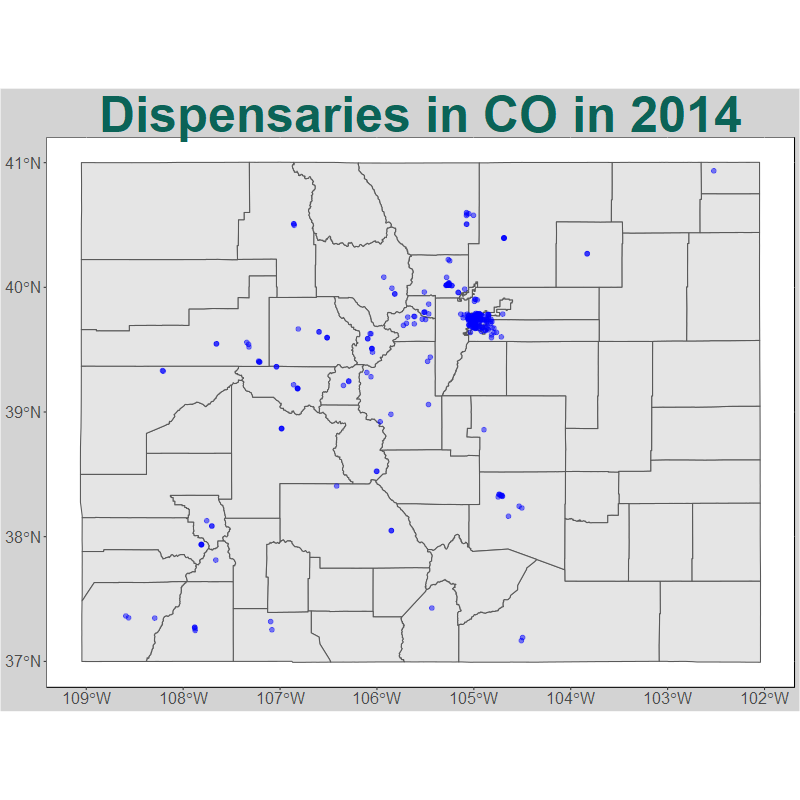
\includegraphics[width=.5\linewidth]{point_map_CO_2014.png}
	}
	\subfloat{
		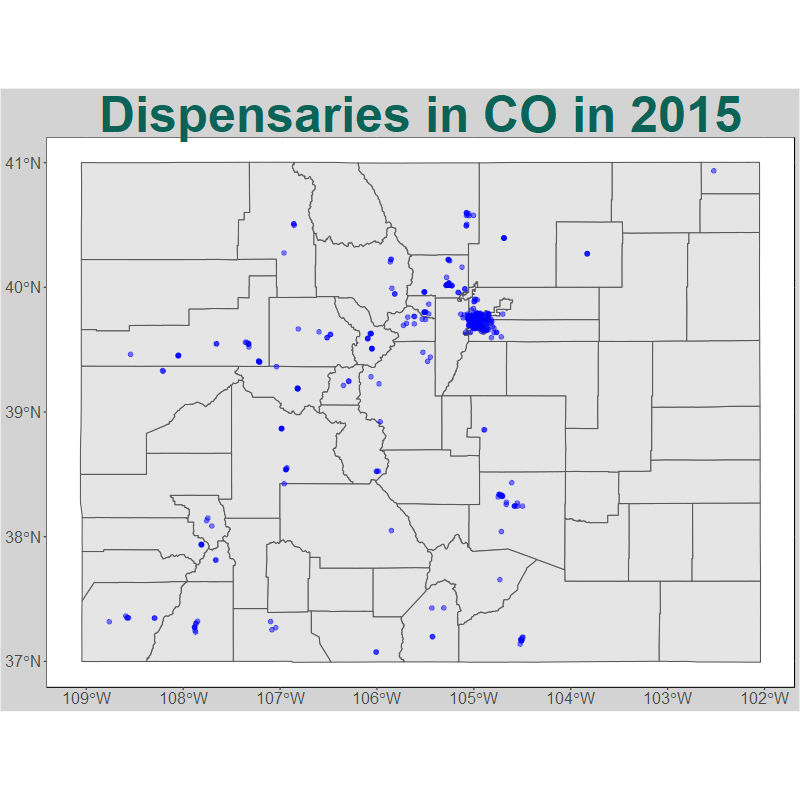
\includegraphics[width=.5\linewidth]{point_map_CO_2015.png}
	}
\newline
	\subfloat{
		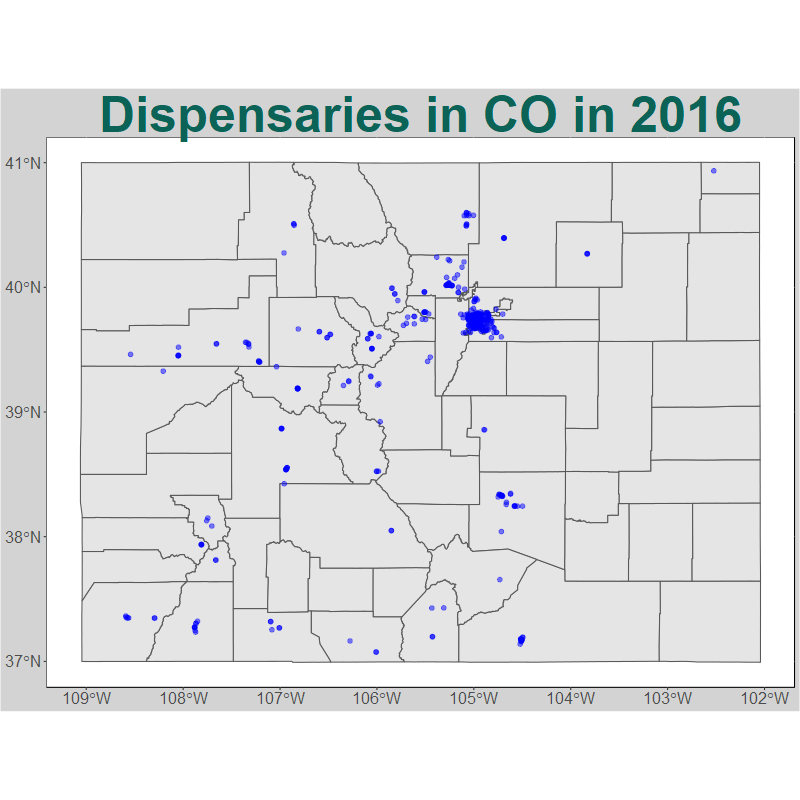
\includegraphics[width=.5\linewidth]{point_map_CO_2016.png}
	}
-
\end{figure}

\begin{figure}[H]
	\centering
	\LARGE{\textbf{Figure 3}}
	\subfloat{
		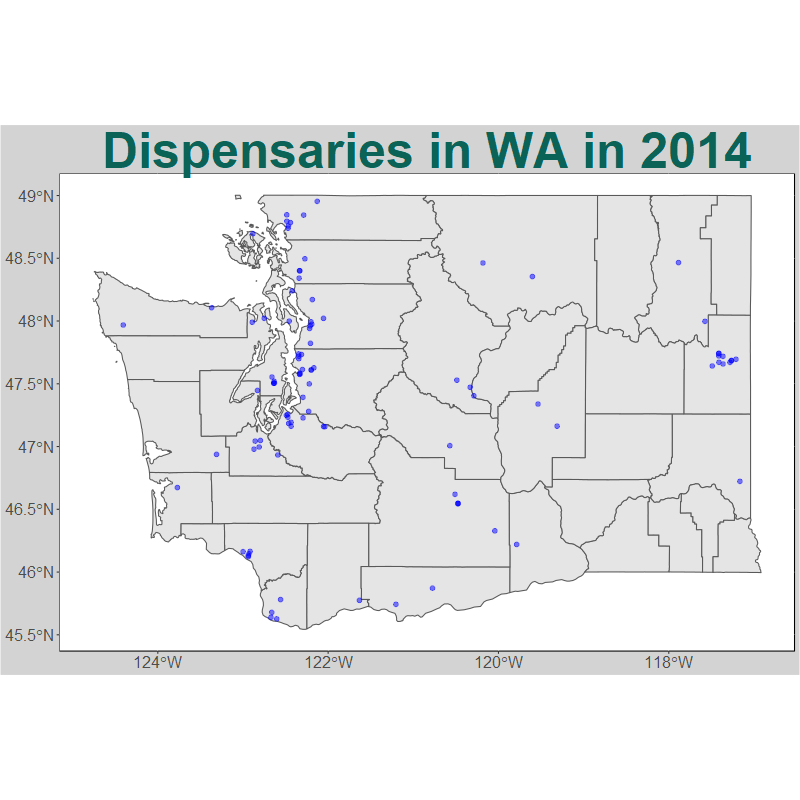
\includegraphics[width=.5\linewidth]{point_map_WA_2014.png}
	}
	\subfloat{
		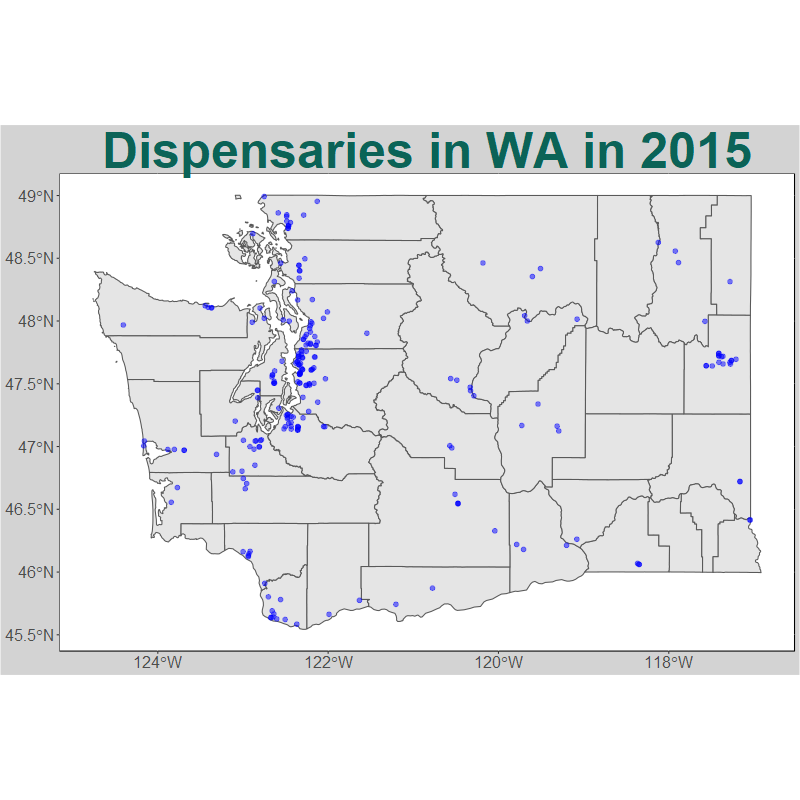
\includegraphics[width=.5\linewidth]{point_map_WA_2015.png}
	}
	\newline
	\subfloat{
		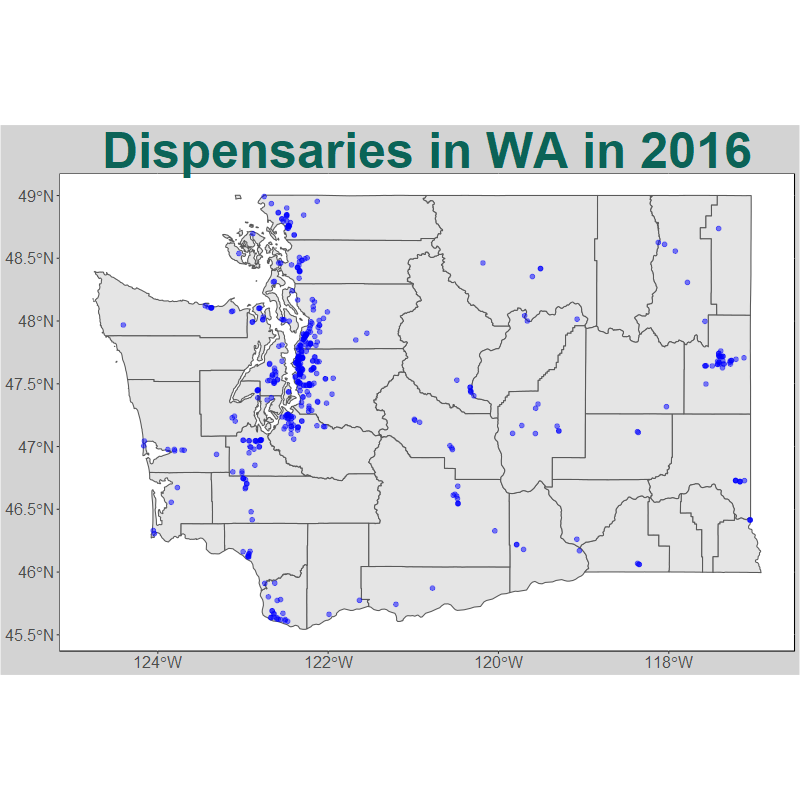
\includegraphics[width=.5\linewidth]{point_map_WA_2016.png}
	}
	-
\end{figure}



%------------------------------------------------------------------------------
% Empirical Analysis
%------------------------------------------------------------------------------

\section{Empirical Analysis}

\subsection{BRFSS Analysis}

My First approach to determine the effect of marijuana legalization on alcohol use is to use the BRFSS survey data along with indicators for changes in state laws. I estimate the following equation using a Tobit model. 

$$
ave\_drinks = \beta_0 +  \beta_1  rec\_l  + \beta_2MML + \bm{\beta_3 Year} + \bm{\beta_4 State} + \bm{\beta_5 Marital} + \bm{\beta_6 Edu} + \beta_7 Smoke
$$

\begin{center}
	\begin{tabular}{||c | c||} 
		\hline
		Variable & Meaning  \\ [0.5ex] 
		\hline\hline
		ave\_drinks & Average Drinks per Week \\ 
		\hline 
		rec\_l & Recreational Consumption is Legal in Respondent's State  \\ 
		\hline
		MML & Medical Marijuana is Legal in Respondent's State  \\
		\hline
		Year & Year Fixed Effects \\
		\hline
		State & State Fixed Effects\\
		\hline
		Marital & Marital Status Dummies  \\ 
		\hline
		Edu & Education level Dummies \\
		\hline
		Smoke & Have you smoked at least 100 cigarettes in your entire life\\[1ex] 
		\hline
	\end{tabular}
\end{center}


The Marital dummies include Married, Divorced, widowed, Separated, Never Married, Member of unmarried couple, refused. Education level is broken up into never attended kindergarten, grades 1-8, grades 9-11, high school graduate, some college or technical school, college graduate, or refused. The dummy for Recreational consumption being legal starts on the first day that laws in each state allowed personal consumption even if no legal dispensaries are open at that time. \par 

I estimate a Tobit Model  \footnote{I considered using a hackmen selection model here instead, but it would not converge. I need to give this model a bit more thought but given the null results I focused more on the spatial analysis below.} because of censoring at Zero. Figure 4 Shows the distribution of respondents average drinks per week. 

\begin{center}
	
	\centering
	\textbf{Figure 4}\par\medskip
	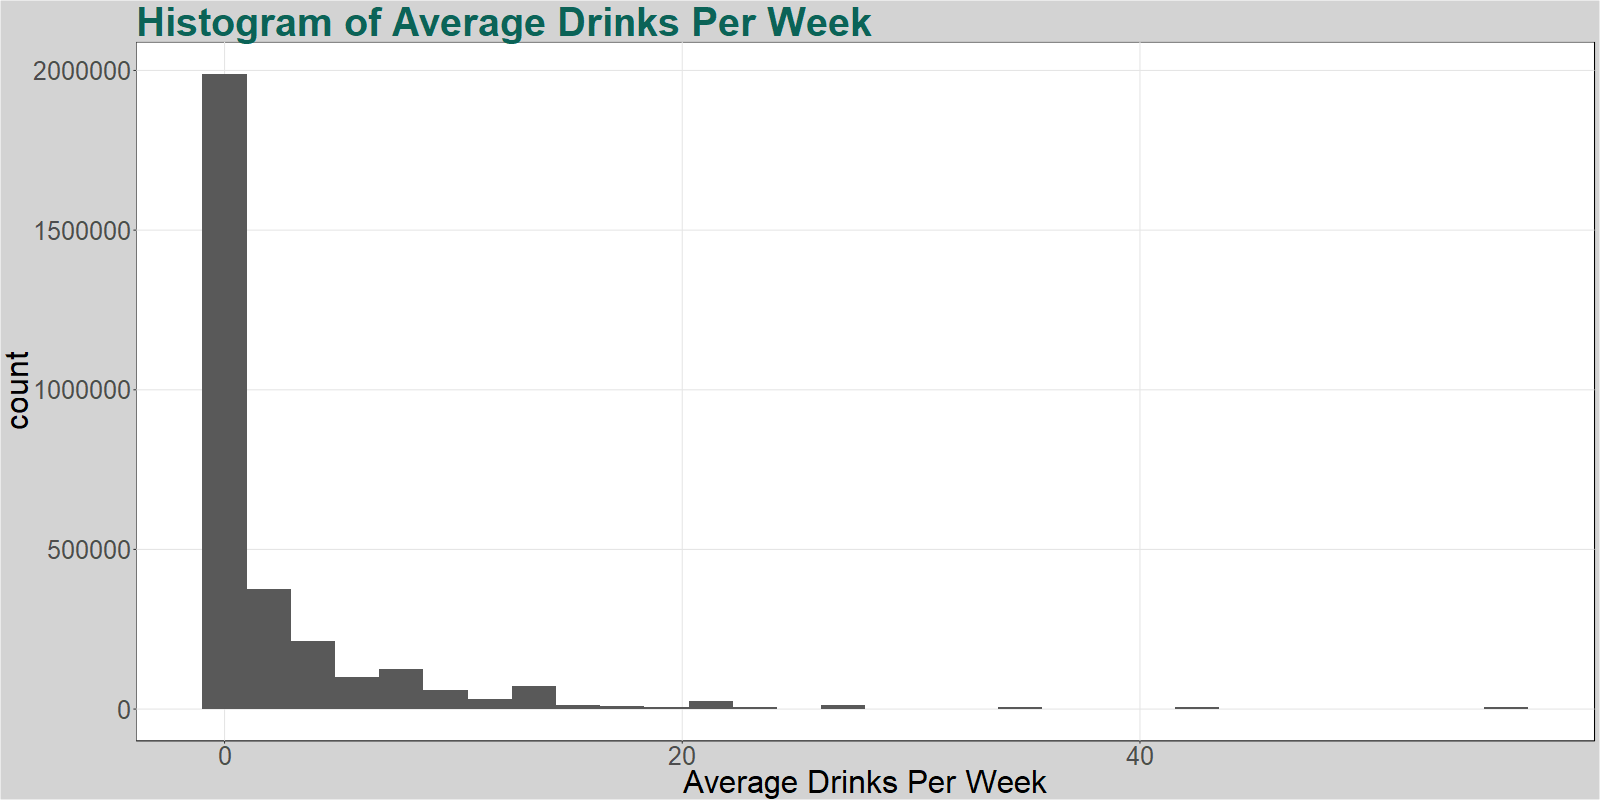
\includegraphics[width=1\linewidth]{Hist_nm_aved_week.png}
\end{center}

Admittedly, the interpretation of this as a Tobit model is a bit non standard. It's not entirely clear what the censored latent variable would be in this case since average weakly drinks is not actually capable of falling below zero. However, McDonald and Moffitt provide a decomposition and interpretation of the Tobit coefficients into ``the effect on the probability of being above zero, and effects conditional upon being above zero" which justifies it's use \cite{Mcdon_moffit}. I also use the survey weights described in the documentation from the CDC \cite{BRFSS_weights}. The coefficients of interest are reported in Table 1 below. 


\begin{center}
	
	\centering
		\LARGE{\textbf{Table 1}}\par\medskip
		
	\normalsize{\textbf{BRFSS Tobit Coefficient of Interest}}\par\medskip
	\scalebox{1}{
		\begin{tabular}{l*{1}{c}}
\hline\hline
            &\multicolumn{1}{c}{Average Drinks Per Week}\\
\hline
&            \\
Recreational Consumption is Legal in Respondent's State       &      0.0148\\
            &     (0.0495)\\
[1em]
Medical Marijuana is Legal in Respondent's State         &       -0.0147\\
            &     (0.0374)\\
\hline
\(N\)       &     3023271\\
\hline\hline
\end{tabular}

	}
\end{center}

The results for both coefficients are statistically insignificant. While I think the idea of using survey data is attractive the model design does not give us very much power. The only variation we can observe is at the state level. Furthermore, we can't use the variation in access within the state because the data only reports the respondents state. It is also possible that there is simply no relationship, and these results suggest at the very least there is not an overwhelming impact. These results give us motivation for turning to the Nielsen scanner data.  The assumptions here are pretty strong, and we are still getting null results. It suggests to me that we need a measure with less measurement error and also includes more variation if we want to detect a relationship. Finer geographic data will provide more variation and directly measuring sales is a more precise but less accurate measure of overall consumption. 


\subsection{Nielson Scanner analysis}

Using the Neislon scanner data in addition to the geographic dispensary data I put together an unbalanced panel of counties across 67 months of observations. This panel includes, for each month and county, the total sales of alcohol in a given county. Using the monthly dispensary addresses, the geocodes, and the census county shapefiles, I also get the number of dispensaries in each county in each month. This gives additional variation in access to marijuana within a state where it is legalized. While having marijuana dispensaries in my county will make it easier for me to purchase marijuana, having dispensaries in neighboring counties or even states will also lower the cost of obtaining marijuana. To capture this effect, I also created a metric for a county?s exposure to nearby dispensaries. This metric is a slightly modified version of the metric used by Shoumitro Chatterjee. \cite{Shoumitro} The formula is below. The index for a county is $c$ and for a dispensary it is $i$. par

$$ \text{Dispensary Distance Metric}_c = \sum_{i=1}^{n} \left( \frac{1}{distance_{ci}}\right)\mathbbm{1} \{distance_{ci} > 1 \} + \mathbbm{1}\{distance_{ci} \le 1 \} 
$$

In words what I am doing is for each county I first find the distance between every dispensary and that county. I then sum one over the distance to that county from every dispensary. Additionally, I round any distances less than one up to one. A dispensary right on the boarder that is less than a mile away from a county is extremely similar to one that is a mile away, but this metric would explode as the distance approaches zero. Rounding distances less than one avoids these extreme outliers. My sample includes dispensaries from around the entire country. So, it may not make sense to give any weight to dispensaries beyond a certain distance. I also create versions of this metric that only include distances less than 1000, 500, and 250 miles. These are V2, V3, and V4 respectively. \par 
 

In my regressions I include the state level policy variations, the number of dispensaries in a county, one the versions of the distance metric and the distance metric interacted with legalized marijuana. I include the interaction term for the dispensary distance metric and marijuana being legal because living near dispensaries likely has different impacts on consumers if it is legal to bring marijuana back to your county of residence compared to it being illegal. I also use log sales so that the coefficients can be interpreted in terms of percent changes rather than levels. I cluster standard errors at the county level to account for correlation of observations within a county. The regression equation is laid out explicitly below and the results are in table 2 below. 

$$
ln\_monthly\_alc\_sale = \beta_0 +  \beta_1  n\_disp  + \beta_2 rec\_l + \beta_3 disp\_dist\_m + \beta_4 disp\_dist\_m*rec\_l + \bm{\beta_5 Year} + \bm{\beta_6 County}$$

\begin{center}
	\begin{tabular}{||c | c||} 
		\hline
		Variable & Meaning  \\ [0.5ex] 
		\hline\hline
		ln\_monthly\_alc\_sale & Log Monthly Alcohol Sales for this County \\ 
		\hline 
		n\_disp & Number of dispensaries in This County  \\ 
		\hline
		rec\_l & Recreational Consumption is Legal in Respondent's State  \\ 
		\hline
		disp\_dist\_m & Dispensary Distance Metric Outlined Above \\
		\hline
		disp\_dist\_m*rec\_l & Dispensary Distance Metric Interacted With Legal Marijuana\\
		\hline
		Year & Year Fixed Effects \\
		\hline
		County & County Fixed Effects\\[1ex] 
		\hline
	\end{tabular}
\end{center}


\begin{center}
	
	\centering
	\LARGE{\textbf{Table 2}}\par\medskip
	
	\normalsize{\textbf{Nielson Scanner Regressions}}\par\medskip
	\scalebox{.8}{
		% latex table generated in R 3.5.1 by xtable 1.8-3 package
% Mon Dec 17 10:42:49 2018
\begin{tabular}{lllllllll}
  \hline
Term & M1 Est & M1 SE & M2 Est & M2 SE & M3 Est & M3 SE & M4 Est & M4 SE \\ 
  \hline
Marijuana Legal to Consume & 0.2289 & 0.0361 & 0.1808 & 0.0323 & 0.1537 & 0.0316 & 0.1412 & 0.0317 \\ 
  Number of Dispensaries & -0.0019 & 0.0014 & -0.0023 & 0.0012 & -0.0024 & 0.0011 & -0.0025 & 0.001 \\ 
  Dispensary Distance Metric & 0.2082 & 0.0465 &  &  &  &  &  &  \\ 
  Dispensary Distance Metric X Marijuana Legal to Consume & -0.2073 & 0.0461 &  &  &  &  &  &  \\ 
  Dispensary Distance Metric V2 &  &  & 0.1609 & 0.0367 &  &  &  &  \\ 
  Dispensary Distance Metric V2 X Marijuana Legal to Consume &  &  & -0.1612 & 0.0366 &  &  &  &  \\ 
  Dispensary Distance Metric V3 &  &  &  &  & 0.1467 & 0.0492 &  &  \\ 
  Dispensary Distance Metric V3 X Marijuana Legal to Consume &  &  &  &  & -0.1475 & 0.0492 &  &  \\ 
  Dispensary Distance Metric V4 &  &  &  &  &  &  & 0.0998 & 0.0698 \\ 
  Dispensary Distance Metric V4 X Marijuana Legal to Consume &  &  &  &  &  &  & -0.1007 & 0.0698 \\ 
  Year FE & Yes & Yes & Yes & Yes & Yes & Yes & Yes & Yes \\ 
  County FE & Yes & Yes & Yes & Yes & Yes & Yes & Yes & Yes \\ 
   \hline
\end{tabular}

	}
\end{center}

Models one through 4 are the same except they use the alternate versions of the distance metric. In each case the point estimates suggest that Marijuana being legal leads to higher alcohol sales while the number of dispensaries leads to less. We Also see an increase in sales with the distance metric. That is the more retail marijuana dispensaries there are near your county the more alcohol you sell, however the effect is only present in states where marijuana is illegal \footnote{The coefficient on the interaction term is roughly equal to the coefficient on the distance metric in each model. If marijuana is legal then the sum of these two coefficients roughly cancel out}. The positive and significant coefficient on the distance metric suggests that there are spillover effects to counties outside of states where marijuana is legalized. In the first model the number of dispensaries is not statistically significant. Suggesting that the primary effect of marijuana legalization was to lead to more alcohol sales. However, models 2, 3, and 4 all have a significant negative coefficient on the number of dispensaries. \par 

The coefficient on the number of dispensaries is hard to square with the other results. What it suggests is that being in a state where marijuana is legal increases alcohol consumption, or being in a nearby county where marijuana is illegal but is next to one with lots of dispensaries close by also increases alcohol consumption. However, actually adding more dispensaries to your own county decreases consumption. While this doesn't make much sense if we think of this as a consistent global parameter, it is possible that there are different types of consumers who have different values for their cross price elasticity of marijuana and alcohol. Some consumers may view marijuana and alcohol as compliments and others as substitutes. Perhaps those who view them as compliments are more responsive to small policy changes (i.e. effective price changes). That is if marijuana is simply legalized or if dispensaries open up in a nearby state, even if it remains illegal in their own state, these types of consumers will respond by increasing consumption of both goods. However, other types of consumers may view them as substitutes. These consumers may also be less responsive to policy (effective price) changes. They don't change their behavior much due to general legalization, and they will not drive to the next county to get marijuana, but if a dispensary is actually opened up in their neighborhood they will start to substitute marijuana for alcohol. This is just speculation, but it could explain the result. \par


These results suggest that the parameter of interest, marijuana and alcohol complementarity, is heterogeneous across agents. This means the interpretation of these results as a sign on the true cross price elasticity that is generalizable across the population is likely incorrect. These coefficients should rather be considered policy specific effects at the county level. That is, they describe the overall impact on the treated population within a given county. That effect may vary if a different state has a different composition of the consumer types I outlined above. Another example is that it is possible that a county that legalizes Marijuana sees an increase in alcohol sales because of an influx of marijuana tourists or young immigrants that are the types of consumers who have a preference for more marijuana and alcohol. \par 

This is not necessarily a problem, but it is important to put the interpretation of these results in perspective. These results might have more external validity if we are considering legalization for a given state in an area without many other legalized states nearby and with populations comparable to Colorado and Washington. For example, Michigan might make an okay comparison. It is perhaps less valid if we are considering a national policy where we would not want to consider immigration or tourism between states in our overall effect, and where the makeup of different types of consumers may be significantly different. This point still applies if I estimated the elasticity like Miller and Seo and applies to their results as well \cite{miller_seo_2018}. If the parameter is heterogeneous than the makeup of the population treated is going to matter. \par

To get a better sense of scale for these coefficients, Table 3 shows a breakdown of the number of dispensaries for counties in Washington and Colorado after 2014. Table 4 shows a similar breakdown for the distance metric for states without legal marijuana after 2014. 

\begin{center}
	
	\centering
	\LARGE{\textbf{Table 3}}\par\medskip
	
	\normalsize{\textbf{Number of Dispensaries in CO and WA after 2014}}\par\medskip
	\scalebox{.8}{
		% latex table generated in R 3.5.1 by xtable 1.8-3 package
% Mon Dec 17 12:46:47 2018
\begin{tabular}{lc}
  \hline
statistic & Value \\ 
  \hline
Min. & 0.00 \\ 
  1st Qu. & 0.00 \\ 
  Median & 1.00 \\ 
  Mean & 5.10 \\ 
  3rd Qu. & 4.00 \\ 
  Max. & 197.00 \\ 
   \hline
\end{tabular}

	}
\end{center}

\begin{center}
	
	\centering
	\LARGE{\textbf{Table 4}}\par\medskip
	
	\normalsize{\textbf{Distance Metric outside of CO and WA after 2014}}\par\medskip
	\scalebox{.8}{
		% latex table generated in R 3.5.1 by xtable 1.8-3 package
% Mon Dec 17 12:46:45 2018
\begin{tabular}{lc}
  \hline
statistic & Value \\ 
  \hline
Min. & 0.05 \\ 
  1st Qu. & 0.32 \\ 
  Median & 0.49 \\ 
  Mean & 0.61 \\ 
  3rd Qu. & 0.75 \\ 
  Max. & 13.52 \\ 
   \hline
\end{tabular}

	}
\end{center}

The coefficients seem to be in a reasonable range for the median or mean of either variable, but the extreme values do not seem as reasonable. For example a distance metric of 13.5 is associated with a 281\% increase in alcohol sales. I should consider nonlinear specification that might give me a better fit along the entire support of the data. 




%------------------------------------------------------------------------------
% Future work and Conclusion
%------------------------------------------------------------------------------

\section{Future Work and Conclusion }
While I see a lot of potential in the panel dataset I have put together, the empirical approach, modeling assumptions, and interpretation of my results all have room for improvement. I need to think more about the exogeneity assumptions I make and the implications of those not holding. I would like to find some more research that uses similar methods so I can get a better understanding of the assumptions and implications and also other robustness checks or data visualization techniques I could employ. I would also like to investigate alternative measure of market exposure other than my ``dispensary distance metric". The add hoc truncations aren't ideal.  \par

I also see some concrete ways that I could make improvements. For example including alcohol tax rates to control for policy shocks in each market. This is an especially legitimate concern for Washington as Miller and Seo bring up the issue of alcohol price changes that correspond with legalization \cite{miller_seo_2018}. \par

I would also like to Run the Neilson Scanner regressions on just Colorado and it's surrounding states and just Washington and it's surrounding states. My results suggest there is heterogeneity in the parameter of interest and so the treated population is going to impact the results. If both of these states have similar results on their own it suggests that the treated population did not differ significantly across these two states. This would support the external validity of my findings. \par

Overall, my findings suggest heterogeneity in the impact of marijuana legalization and access on alcohol consumption. They also suggest that, in the case of Colorado and Washington, recreational legalization increased retail alcohol sales while opening dispensaries decreased alcohol sales in their own county and increased alcohol sales in counties of other states. The Retail scanner analysis gives a precise look into the impact on the treated populations of Colorado and Washington. in theory, individual level variables like those in the BRFSS data could be used to control for differences in populations and arrive at estimates of this effect for specific populations. However, the level of precision in the BRFSS data is too low to detect any statistically significant relationships. Additional work is need both in my paper and in the broader literature to more thoroughly understand how recreational marijuana legalization and readily accessible marijuana will impact alcohol consumption. 
 
%------------------------------------------------------------------------------
% bib
%------------------------------------------------------------------------------
\bibliographystyle{apacite}
\bibliography{References}


%------------------------------------------------------------------------------
% Appendix 
%------------------------------------------------------------------------------

\section{Appendix}

\subsection{Appendix A}

\begin{figure}[H]
	\centering
	\LARGE{\textbf{Counties in Scanner Panel Per Month}}\par\medskip
	\scalebox{.6}{
	% latex table generated in R 3.5.1 by xtable 1.8-3 package
% Mon Dec 17 02:10:42 2018
\begin{tabular}{llr}
  \hline
year & month & Number of Counties \\ 
  \hline
2011 & 01 & 1806 \\ 
  2011 & 02 & 1807 \\ 
  2011 & 03 & 1812 \\ 
  2011 & 04 & 1812 \\ 
  2011 & 05 & 1813 \\ 
  2011 & 06 & 1817 \\ 
  2011 & 07 & 1867 \\ 
  2011 & 08 & 1872 \\ 
  2011 & 09 & 1868 \\ 
  2011 & 10 & 1871 \\ 
  2011 & 11 & 1871 \\ 
  2011 & 12 & 1875 \\ 
  2012 & 01 & 1847 \\ 
  2012 & 02 & 1836 \\ 
  2012 & 03 & 1875 \\ 
  2012 & 04 & 1874 \\ 
  2012 & 05 & 1891 \\ 
  2012 & 06 & 1888 \\ 
  2012 & 07 & 1884 \\ 
  2012 & 08 & 1881 \\ 
  2012 & 09 & 1893 \\ 
  2012 & 10 & 1882 \\ 
  2012 & 11 & 1881 \\ 
  2012 & 12 & 1876 \\ 
  2013 & 01 & 1863 \\ 
  2013 & 02 & 1844 \\ 
  2013 & 03 & 1853 \\ 
  2013 & 04 & 1854 \\ 
  2013 & 05 & 1864 \\ 
  2013 & 06 & 1900 \\ 
  2013 & 07 & 1900 \\ 
  2013 & 08 & 1881 \\ 
  2013 & 09 & 1879 \\ 
  2013 & 10 & 1873 \\ 
   \hline
\end{tabular}

}
	\scalebox{.6}{
	% latex table generated in R 3.5.1 by xtable 1.8-3 package
% Mon Dec 17 02:10:42 2018
\begin{tabular}{llr}
  \hline
year & month & Number of Counties \\ 
  \hline
2013 & 11 & 1884 \\ 
  2013 & 12 & 1887 \\ 
  2014 & 01 & 1858 \\ 
  2014 & 02 & 1862 \\ 
  2014 & 03 & 1866 \\ 
  2014 & 04 & 1868 \\ 
  2014 & 05 & 1878 \\ 
  2014 & 06 & 1890 \\ 
  2014 & 08 & 1889 \\ 
  2014 & 09 & 1888 \\ 
  2014 & 10 & 1885 \\ 
  2014 & 11 & 1893 \\ 
  2014 & 12 & 1892 \\ 
  2015 & 01 & 1878 \\ 
  2015 & 02 & 1883 \\ 
  2015 & 03 & 1895 \\ 
  2015 & 04 & 1905 \\ 
  2015 & 05 & 1919 \\ 
  2015 & 06 & 1926 \\ 
  2015 & 07 & 1940 \\ 
  2015 & 08 & 1950 \\ 
  2015 & 09 & 1964 \\ 
  2015 & 10 & 1956 \\ 
  2015 & 11 & 1952 \\ 
  2015 & 12 & 1948 \\ 
  2016 & 01 & 1945 \\ 
  2016 & 02 & 1936 \\ 
  2016 & 03 & 1934 \\ 
  2016 & 04 & 1941 \\ 
  2016 & 05 & 1939 \\ 
  2016 & 06 & 1944 \\ 
  2016 & 07 & 1947 \\ 
  2016 & 08 & 1946 \\ 
   \hline
\end{tabular}

}
\end{figure}


%------------------------------------------------
% end doc
%------------------------------------------------
\end{document}